\section{Analyse von Metadatenstandards} \label{Analyse Datenbestaende}
Nach dem nun die Portale \ac{DRS}, Naturschutz-Bildarchiv und \ac{FADO}, der \ac{LUBW} und das Literaturarchiv der \ac{ICT-ENSURE} im Kapitel \ref{Stand der Technik} genauer betrachtet und die Verwaltungsstrukturen aufgezeigt wurden, betrachtet dieses Kapitel nun Standards f\"ur Metadaten. Hierbei wird unterschieden, ob es sich um fachliche oder technische Metadaten handelt.

\subsection{Fachlich}
Fachliche Metadaten sind Daten, welche den Inhalt einer Datei oder eines Dokuments genauer beschreiben und dem Anwender dabei helfen f\"ur ihn relevante Dateien zu identifizieren. Solche Metadaten sind immer fachspezifisch und unabh\"angig von den technischen Eigenschaften einer Datei.
\cite{Fachliche_Metadaten_Wissensportal_BI} \cite{Fachliche_Metadaten_msg} \cite{DHW_Wiki_Metadaten} \cite{Multimedia_retrieval}

Die Dokumente der Fachsysteme der \ac{LUBW}, sowie der \ac{ICT-ENSURE} enthalten alle fachliche Metadaten. Eine genaue Aufstellung aller fachlichen Metadaten der in dieser Arbeit untersuchten Dokumente ist im Anhang \ref{Metadaten der LUBW Fachsysteme} zu finden.

\subsection{Fachliche Metadaten-Standards} \label{Fachliche Metadaten-Standards}
F\"ur die Erstellung eines Datenkonzepts wie es im Kapitel \ref{Erstellung eines Datenkonzepts} geschieht, ist es aber nicht nur notwendig die vorhandenen Metadaten zu betrachten. Auch Standards f\"ur fachliche Metadaten sollen in diesem Umfeld untersucht werden.

Da fachliche Metadaten meist anwendungs- beziehungsweise dokumentbezogen sind, gibt es nicht sehr viele Standards, welche sich im Umfeld der \ac{LUBW} beziehungsweise der \ac{ICT-ENSURE} einsetzen lassen.

\subsubsection{Darwin Core}
Darwin Core beschreibt eine Zusammenfassung von Metadaten, welche f\"ur biologische Zwecke eingesetzt werden k\"onnen. So ist es zum Beispiel m\"oglich, Angaben zum Organismus oder zum Lebensraum zu machen. 

Hierf\"ur verwendet Darwin Core bis zu 172 Tags, welche jedoch nicht zwingend verwendet werden m\"ussen. Zus\"atzlich enth\"alt der Standard auch die Tags von Dublin Core (siehe Abschnitt \ref{Dublin Core}) um das Dokument grundlegend zu beschreiben.
\cite{Darwin_Core} \cite{Wiki_Darwin_Core}

Ii Listing \ref{Darwin Core Beispiel in XML}\footnote{\url{http://rs.tdwg.org/dwc/terms/guides/xml/index.htm}} ist einmal ein Beispiel f\"ur den Darwin Core-Standard  mit XML dargestellt. Es ist zu sehen, das ein "`SimpleDarwinRecord"' verwendet wird, welcher nicht alle 172 Tags beinhaltet. 

Es ist auch zu erkennen, dass die Dublin Core-Tags inbegriffen sind (beginnend mit "`dcterms"'). Die eigentliche Tags des Darwin-Standards beginnen mit "`dwc"'.
\lstinputlisting[caption=Darwin Core-Beispiel in XML, label=Darwin Core Beispiel in XML]{Code/Darwin_Core.xml}

\subsubsection{INSPIRE} \label{INSPIRE}
\ac{INSPIRE} ist ein Standard f\"ur Metadaten, welcher von der \ac{EU} nach der Richtlinie "`2007/2/EG"' vom 14. M�rz 2007 erlassen wurde. \ac{INSPIRE} enth\"alt Metadaten, welche f\"ur Geo-Referenzen benutzt werden m\"ussen, denn nach der eben genannten \ac{EU}-Richtlinie m\"ussen alle vom Land ver\"offentlichten digitalen Dateien mit Geo-Referenzen versehen werden.

\ac{INSPIRE} stellt 25 Meta-Tags zur Verf\"ugung, mit dessen Hilfe die \ac{EU}-Richtlinie zur Bekanntmachung von Geo-Referenzen eingehalten wird.
Au\ss{}erdem enth\"alt der \ac{INSPIRE}-Standard die notwendigen Tags der DIN EN ISO 19115 (siehe Abschnitt \ref{ISO 19115}), wodurch dieser gleichzeitig nach dieser Norm ISO-konform wird. 
\cite{INSPIRE_Richtlinie}

Von den 25 Meta-Tags m\"ussen 12 Tags zwingend angegeben werden, um die Richtlinie zu erf\"ullen. Die Meta-Tags von \ac{INSPIRE} sind zum Teil untergliedert, was bedeutet, dass eine Vielzahl mehr an Information in diesen Standard enthalten sein k\"onnen.

Aus \"Ubersichlichkeitsgr\"unden wird an dieser Stelle kein Beispiel Listing erfolgen, da das XML-Format von \ac{INSPIRE} sehr ausf\"uhrlich und gro\ss{} ist. Es wird jedoch an dieser Stelle auf den Editor f\"ur \ac{INSPIRE}-Metadaten der Europ\"aischen Kommission verwiesen, mit dessen Hilfe schnell und einfach XML-Dokumente mit \ac{INSPIRE}-Metadaten erzeugt werden k\"onnen\footnote{\url{http://inspire-geoportal.ec.europa.eu/editor/}}.
\cite{INSPIRE_Geoportal} \cite{Wiki_Inspire} 

\subsubsection{DIN EN ISO 19115} \label{ISO 19115}
Die DIN EN ISO 19115 ist eine Norm, welche 2005 spezifiziert wurde. Sie enth\"alt Metadaten f\"ur die Bescheibung von Geo-Information. Mit \"uber 400 m\"oglichen Tags ist sie eine der detailliertesten Beschreibungsstandards f\"ur Geo-Daten. 

Von den \"uber 400 Tags sind f\"ur eine Verwendung der Norm nur ca. 22 Tags erforderlich. Alle anderen Tags sind optional.
\cite{ISO_19115_Doku} \cite{Wiki_ISO_19115}

Wird der \ac{INSPIRE}-Standard verwendet (siehe Abschnitt \ref{INSPIRE}), so ist automatisch auch die ISO 19115 erf\"ullt, da diese Bestandteil  von \ac{INSPIRE} ist.
\cite{INSPIRE_Richtlinie}

\subsubsection{ONIX}
Der \ac{ONIX}-Standard ist international bekannt und f\"ur den elektronischen Austausch von Buchinformationen geschaffen worden.

\ac{ONIX} kann gem\"a\ss{} der Lizenz frei verwendet werden und ist zur Beschreibung von traditionellen B\"uchern und E-Books vorgesehen.
Der Standard enth\"alt sehr viele Tags, mit dessen Hilfe ein Buch beschrieben werden kann. So k\"onnen zum Beispiel Angaben zum Verleger und zur ISBN gemacht werden. \cite{ONIX} \cite{Wiki_ONIX}

Nachteilig ist, dass das Format sehr viel auf Abk\"urzungen setzt, was eine Menschenlesbarkeit  erschwert oder gar verhindert.

Ein kleines Beispiel zum \ac{ONIX}-Format ist im Listing \ref{ONIX Beispiel in XML} zu finden. Hier wird kurz beschrieben das es sich um einen Download handelt, welcher im Epub-Format vorhanden und lesbar ist. Ohne die Erkl\"arungen am Ende der Zeile w\"aren die Informationen nicht ohne weitere Hilfe lesbar. 

\lstinputlisting[caption=ONIX-Beispiel in XML, label=ONIX Beispiel in XML]{Code/ONIX.xml} \cite{ONIX_Example}


\subsection{Technisch}
Technische Metadaten sind Daten, die den internen Dateiaufbau und dessen Inhalt beschreiben. Sie betreffen den Anwender nur sekund\"ar und sind eher wichtig f\"ur die richtige Speicherung und f\"ur Administratoren. Technische Metadaten sind unabh\"angig von dem fachlichen Inhalt eines Dokuments und beschreiben zum Beispiel dessen Datenformat, das Erstellungsdatum oder die Nutzerrechte genauer.
\cite{Fachliche_Metadaten_Wissensportal_BI} \cite{Fachliche_Metadaten_msg} \cite{DHW_Wiki_Metadaten} \cite{Multimedia_retrieval}

In den Systemen der \ac{LUBW} und der \ac{ICT-ENSURE} werden keine technischen Metadaten angezeigt, weshalb diese an der Stelle nicht betrachtet werden.
Technische Metadaten sind vor allem bei physikalischen Daten wichtig. Da die Systeme nur intern mit diesen Daten arbeitenm werden sie dem Nutzer nicht angezeigt. In einem \ac{ECM}-System spielen sie jedoch eine wichtige Rolle und werden im sp\"ateren Verlauf der Arbeit genauer betrachtet. 

Ref?????

\subsection{Technische Metadaten-Standards}
Wie schon bei den fachlichen Metadaten (siehe Abschnitt \ref{Fachliche Metadaten-Standards}) gibt es auch f\"ur technische Metadaten Standards, welche versuchen, die Beschreibung von Dokumenten zu vereinheitlichen. In den folgenden Abschnitten werden nun einige Standards f\"ur technische Metadaten vorgestellt und genauer beschrieben.

\subsubsection{Dublin Core} \label{Dublin Core}
Dublin Core ist ein Standard, welcher ein Dokument grundlegend beschreibt. Von der \ac{DCMI}, welche den Standard beschlossen, hat werden 15 Kernfelder zur Verwendung, die so genannten "`core elements"', empfohlen. Es gibt jedoch weitere Felder, welche zus\"atzliche Informationen enthalten k\"onnen.
\cite{Wiki_Dublin_Core} \cite{Dublin_Core} \cite{Multimedia_retrieval}

Der Standard sollte heute Bestandteil jeder Website sein, da viele Suchmaschinen wie zum Beispiel Google nach Dublin Core-Metadaten suchen und Ergebnisse zum Beispiel anhand dieser Filtern. Ist also eine \ac{SEO} angedacht beziehungsweise wie in \ac{FADO} umgesetzt, sollten diese Metadaten vorhanden sein.
\cite{Dublin_Core_und_SEO}

Ein Beispiel f\"ur Dublin Core ist im Listing \ref{Dublin Core Beispiel in HTML}\footnote{\url{http://de.wikipedia.org/wiki/Dublin_Core}} zu finden. Hier wird der Standard im HTML-Format verwendet. Es wird zum einen auf das offizelle Schema verlinkt, zum anderen werden die einzelnen Metadaten dargestellt, welche in den Meta-Tags zu finden sind, und mit dem Namen "`DC."' beginnen, um zu verdeutlichen, dass es sich hier um Dublin Core handelt.

\lstinputlisting[caption=Dublin Core-Beispiel in HTML, label=Dublin Core Beispiel in HTML]{Code/Dublin_Core.html}

\subsubsection{Exif} \label{Exif}
Das Exif-Metadatenformat ist ein Standard f\"ur die Beschreibung von Bildern. In der heutigen Zeit verf\"ugen nahezu alle digitalen Kameras \"uber dieses Format und speichern bei der Aufnahme eines Bildes verschiedene Parameter im \ac{Exif} ab. 
\cite{Wiki_Exif}

Mit \"uber 50 Tags kann ein Bild mit Hilfe von \ac{Exif} sehr detailiert beschrieben werden. Es gibt unter anderem Tags f\"ur die Belichtungszeit, die Blende und den Farbraum. Aber auch Koordinaten, an dem das Bild aufgenommen wurde, k\"onnen vorhanden sein.
\cite{Wiki_Exif} \cite{Exif_Spezifikation}

Eine genaue Auflistung aller Tags und deren Inhalt ist in der Spezifikation "`Exchangeable Image File Format for digital still cameras"'\footnote{\url{http://www.jeita.or.jp/japanese/standard/book/CP-3451C_E/\#page=1}} zum Format zu finden.

\subsubsection{RDF} \label{Rdf}
Das \ac{RDF} ist im eigentlichen Sinn keine Beschreibung von standardisierten Metadaten. Vielmehr ist es ein \"ubergeordneter Standard, der beschreibt, wie Metadaten beschrieben werden k\"onnen.
\cite{Wiki_RDF}

Hierf\"ur wird eine Satzstruktur verwendet, welche jeweils aus Subjekt, Pr\"adikat und Objekt besteht. Am folgenden Beispiel in Abbildung \ref{RDF Struktur} wird verdeutlicht, was genau mit einer Satzstruktur gemeint ist. \cite{Multimedia_retrieval}

\begin{figure}[!ht]
\centering
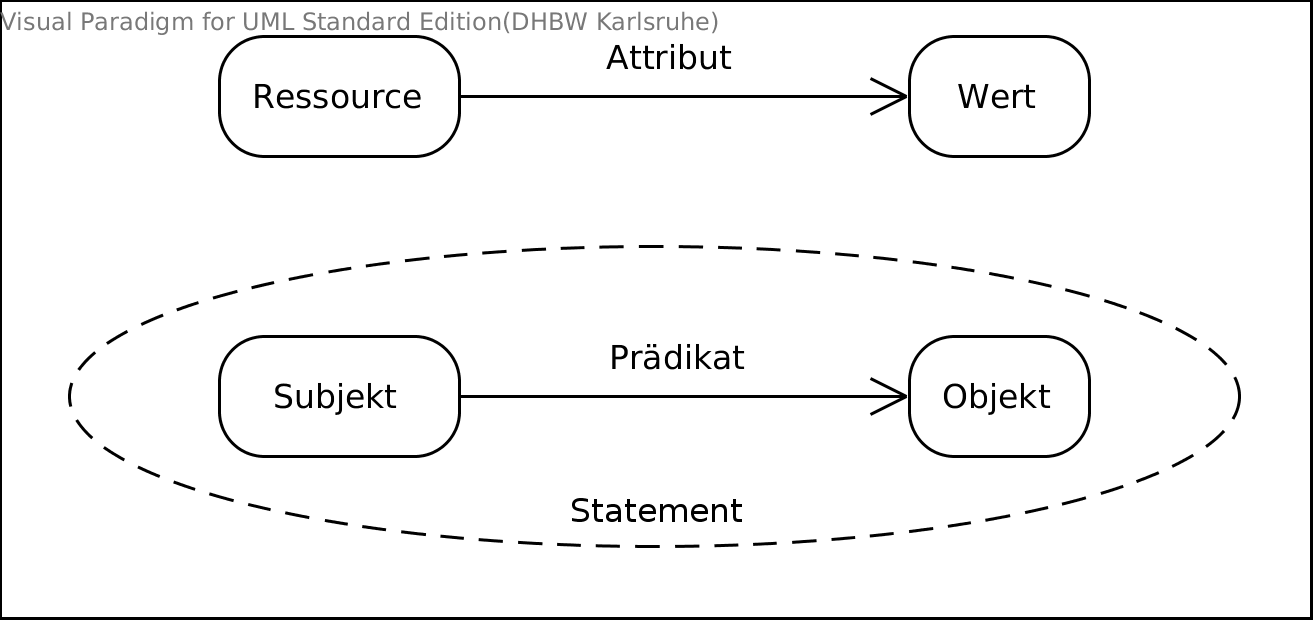
\includegraphics[width=8cm]{Bilder/RDF.png}
\caption{Struktur von \ac{RDF}}
\label{RDF Struktur}
\centering
\end{figure}

Mit Hilfe von \ac{RDF} kann also ausgesagt werden, dass eine Website "`www.beispiel.com"' ein Erstellungsdatum am 15.06.2015 hat.
Somit ergibt sich die Aufteilung:
\begin{itemize}
 \item Subjekt: www.beispiel.com
 \item Pr\"adikat: hat Erstellungsdatum
 \item Objekt: 15.06.2015
\end{itemize}

In XML w\"urde dieses Beispiel wie im Listing \ref{RDF in XML} aussehen.
\cite{Multimedia_retrieval}

\lstinputlisting[caption=RDF-Beispiel in XML, label=RDF in XML]{Code/RDF.xml}

\subsubsection{ANSI/NISO Z39.87-2006 (R2011)} \label{R2011}
Das ANSI/NISO Z39.87-2006 ist ein amerikanisches nationales Format, welches Bilddateien beschreibt. Es ist \"ahnlich aufgebaut wie \ac{Exif} und enth\"alt grundlegend die selben M\"oglichkeiten wie das im Abschnitt \ref{Exif} vorgestellte \ac{Exif}. \cite{NISO_Standard}

Da sich die Arbeit jedoch mit europ\"aischen Projekten und Organisationen besch\"aftigt, wird auf dieses Format hier nicht weiter eingegangen.